
\section{Introduction}
\label{sec:Introduction}

\subsection{Project objective}

When a voltage is applied to an IPMC it results in a bending motion of the material that can be controlled by adjusting the applied voltage. There is potential for use of actuators in industrial mixing if they are found to be more efficient than traditional mixing blades or rotors, but also for use in accurate muscle replication which is of interest especially in the area of robotics.


The primary objective of this project is to create a definition of 'mixing' and apply this to assess the mixing efficiency of three known actuators using provided video data, the aim of this being to ascertain which actuator is the most efficient at mixing. A number of processes are investigated including actuator motion tracking, system entropy and particle image velocimetry.



\subsection{Source video data}

This research project is focused specifically on three sizes of Nafion IPMC stirrer \cite{dupont}; 112, 117 and 1110, shown in Figure 1. A 300 frame video of each actuator stirring a solution was provided as the source data. The videos show the actuators placed in water scattered with ink drops when a pulsed voltage is applied to them via the discharge of a capacitor inducing oscillatory motion to stir the liquid. A 0.01F capacitor was used for both the 112 and 117 actuators, and a 0.4F capacitor for the 1110. The ink acts as a marker to make the fluid dynamics clearer for analysis, however the quantity of dye used is unknown and inconsistent throughout the videos. The source data from this is in the form of a three dimensional matrix for every frame of the three videos and the physical dimensions are known for one video.


\begin{figure}[h]

	\subfigure[112 actuator]{
		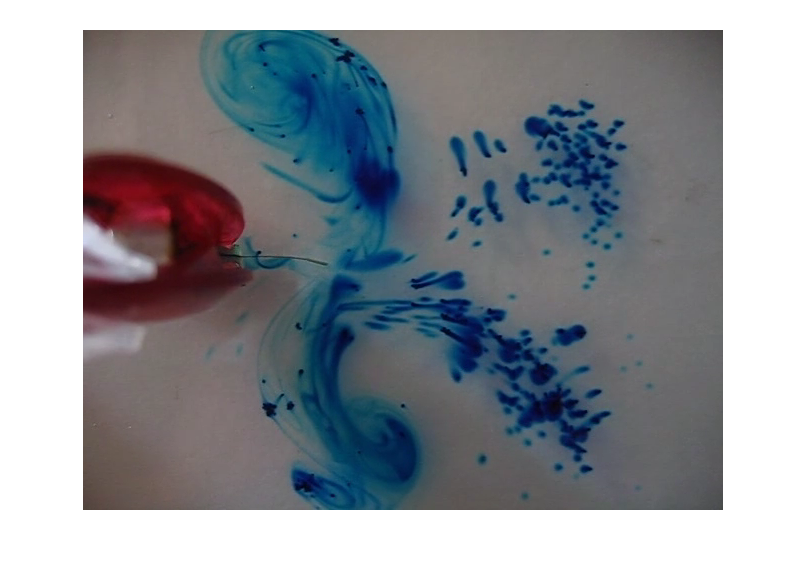
\includegraphics[width=\textheight/3]{Pictures/Small200norm.png}}
	\subfigure[117 actuator]{
		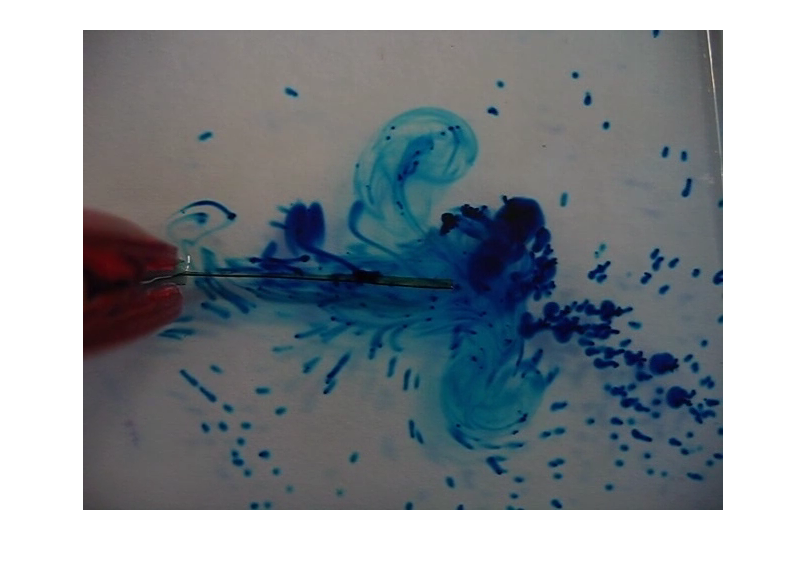
\includegraphics[width=\textheight/3]{Pictures/Med200norm.png}}
    \center
	\subfigure[1110 actuator]{
		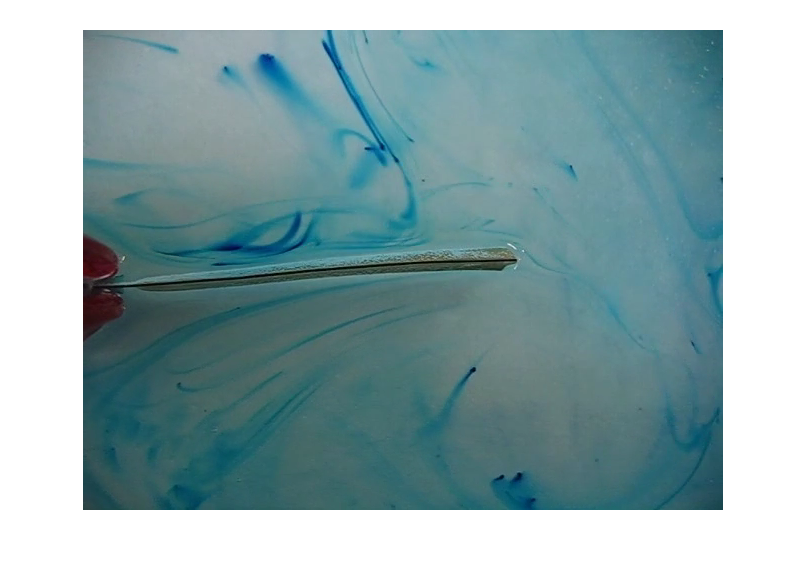
\includegraphics[width=\textheight/3]{Pictures/Large200norm.png}}
     \caption{Frame 200 of each Nafion actuator video.}
\end{figure}

